\documentclass[12pt,a4paper]{article}

\usepackage[margin=2.5cm]{geometry}
\usepackage{amsmath}
\usepackage{amssymb}
\usepackage{graphicx}
\usepackage{booktabs}
\usepackage{hyperref}
\usepackage{xcolor}
\usepackage{listings}

\definecolor{codegray}{RGB}{245,245,245}
\definecolor{codeblue}{RGB}{30,80,140}

\lstset{
  basicstyle=\ttfamily\small,
  backgroundcolor=\color{codegray},
  keywordstyle=\color{codeblue},
  columns=fullflexible,
  keepspaces=true,
  showstringspaces=false,
  frame=single,
  breaklines=true
}

\title{CARD: Correlation Aware Restoration with Diffusion}
\author{Hadi Fathipour}
\date{Tir 1405 (June 2025)}

\begin{document}

\hypersetup{pageanchor=false}
\begin{titlepage}
  \centering
  
\includegraphics[width=3cm]{logo.png}

  \vspace{1cm}
  {\Large\textbf{Research Project \(\cdot\) Digital image processing course}\par}

  \vspace{1cm}
  {\huge\textbf{CARD: Correlation Aware Restoration with Diffusion}\par}

  \vspace{0.4cm}
  \rule{0.85\textwidth}{0.4pt}

  \vspace{1.2cm}
  \begin{tabular}{rl}
    \textbf{Supervisor:} & Hossein ali Ghiassi rad \\
    \textbf{Student:} & Hadi Fathipour -- Student ID: 40411334 \\
    \textbf{Presentation Date:} & Tir 1405 (June 2025) \\
  \end{tabular}

  \vfill
  {\large Image Processing Project\par}
\end{titlepage}
\hypersetup{pageanchor=true}

\pagenumbering{arabic}
\setcounter{page}{1}
\tableofcontents
\newpage

\section{Abstract}

This report describes a compact course implementation inspired by the paper
\textit{CARD: Correlation Aware Restoration with Diffusion}. The original paper
addresses a practical weakness in many image restoration methods: they assume
that image noise is independent and identically distributed Gaussian noise,
while real camera sensors can produce spatially correlated noise. The project
implemented here preserves the central image-processing idea of CARD by
explicitly modeling correlated noise with a covariance matrix and using that
covariance during restoration. The implementation is not a full diffusion or
DDRM reproduction; instead, it is a reproducible CPU-friendly demonstration
based on synthetic correlated noise, covariance whitening, and Wiener-style
restoration.

\section{Problem Statement}

Many denoising and image restoration algorithms assume the measurement model
\[
  y = Hx_0 + n,
  \qquad
  n \sim \mathcal{N}(0, \sigma^2 I),
\]
where \(x_0\) is the clean image, \(H\) is a degradation operator, and \(n\) is
i.i.d. Gaussian noise. In real imaging systems, especially rolling-shutter CMOS
sensors, this assumption is often inaccurate. Sensor readout mechanisms can
create row-wise and neighborhood-level noise correlations.

The correlated-noise model is:
\[
  y = Hx_0 + n,
  \qquad
  n \sim \mathcal{N}(0, \sigma^2 \Sigma),
\]
where \(\Sigma\) is the covariance matrix that describes spatial noise
correlation. If restoration methods ignore \(\Sigma\), they may either leave
structured artifacts in the output or smooth useful image details too heavily.

\section{Original CARD Method}

The CARD paper proposes a training-free extension of DDRM for restoration under
correlated Gaussian noise. The key mathematical step is whitening. Given:
\[
  n \sim \mathcal{N}(0, \sigma^2 \Sigma),
\]
CARD multiplies the measurement equation by \(\Sigma^{-1/2}\):
\[
  \Sigma^{-1/2} y
  =
  \Sigma^{-1/2} Hx_0
  +
  \Sigma^{-1/2} n.
\]
This produces:
\[
  \tilde{y} = \tilde{H}x_0 + \tilde{n},
  \qquad
  \tilde{n} \sim \mathcal{N}(0, \sigma^2 I).
\]

After this transformation, the noise satisfies the i.i.d. assumption required by
DDRM-style restoration. The full paper then modifies DDRM's diffusion updates in
the whitened measurement space.

\section{Implemented Course Version}

The implementation in this project is named \texttt{card}. It keeps the core
idea of CARD but replaces the diffusion sampler with a lightweight
covariance-aware restoration step. This makes the project easy to run on CPU and
suitable for an image processing course demonstration.

\subsection{Project Structure}

\begin{table}[h]
  \centering
  \begin{tabular}{ll}
    \toprule
    File & Responsibility \\
    \midrule
    \texttt{card/noise.py} & covariance model, coloring, whitening, noise generation \\
    \texttt{card/restoration.py} & Gaussian baseline and CARD restoration \\
    \texttt{card/metrics.py} & PSNR and SSIM metrics \\
    \texttt{card/images.py} & synthetic image and output grid generation \\
    \texttt{card/pipeline.py} & complete experiment pipeline \\
    \texttt{main.py} & command-line entry point \\
    \bottomrule
  \end{tabular}
  \caption{Main implementation files.}
\end{table}

\subsection{Pipeline}

The experiment follows these steps:

\begin{enumerate}
  \item Generate a deterministic clean synthetic image.
  \item Construct a rolling-shutter-like covariance matrix.
  \item Use a coloring matrix to generate correlated Gaussian noise.
  \item Add this noise to the clean image.
  \item Restore the noisy image using a Gaussian baseline.
  \item Restore the noisy image using the CARD covariance-aware method.
  \item Compute PSNR and SSIM.
  \item Save a visual comparison image.
\end{enumerate}

\section{Covariance Model}

The project uses square patches of size \(p \times p\). For each pixel pair
\(i,j\) inside a patch, the covariance is defined by row and column distance:
\[
  \Sigma_{ij}
  =
  \rho^{|r_i-r_j|}
  (0.45\rho)^{|c_i-c_j|}
  +
  \epsilon I,
\]
where:

\begin{itemize}
  \item \(r_i, c_i\) are the row and column coordinates of pixel \(i\);
  \item \(\rho\) controls correlation strength;
  \item \(\epsilon I\) is a small regularization term.
\end{itemize}

This model creates stronger row-wise correlations than column-wise correlations,
which approximates rolling-shutter banding behavior.

\section{Coloring and Whitening}

The covariance matrix is decomposed as:
\[
  \Sigma = Q \Lambda Q^T.
\]

The coloring transform is:
\[
  C = Q\Lambda^{1/2}Q^T.
\]
It maps standard Gaussian noise \(z \sim \mathcal{N}(0,I)\) into correlated
noise:
\[
  n = \sigma C z.
\]

The whitening transform is:
\[
  W = Q\Lambda^{-1/2}Q^T.
\]
It maps correlated noise back toward an i.i.d. representation:
\[
  W \Sigma W^T \approx I.
\]

\section{CARD Restoration Method}

The CARD restoration function projects noisy patches into the covariance
eigenbasis. In that basis, each coefficient has an estimated signal variance and
noise variance. The method applies Wiener-style shrinkage:
\[
  g_i =
  \frac{\sigma^2_{\text{signal},i}}
  {\sigma^2_{\text{signal},i} + \sigma^2_{\text{noise},i}}.
\]

The restored patch coefficients are:
\[
  \hat{c}_i = g_i c_i.
\]

After reconstruction, the covariance-aware output is blended with a Gaussian
baseline. This Gaussian result acts as a simple image prior in place of the
pretrained diffusion prior used by the original CARD method.

\section{How to Run}

The project uses \texttt{uv} for dependency management.

\begin{lstlisting}[language=bash]
uv sync
uv run python main.py
\end{lstlisting}

The demo writes:

\begin{lstlisting}
results/card_demo.png
\end{lstlisting}

Verification commands:

\begin{lstlisting}[language=bash]
uv run pytest
uv run ruff check .
uv run basedpyright
\end{lstlisting}

\section{Results}

The generated visual result is shown in Figure~\ref{fig:card-result}. The panels
show the clean image, correlated noisy image, Gaussian baseline, and CARD-style
restoration.

\begin{figure}[h]
  \centering
  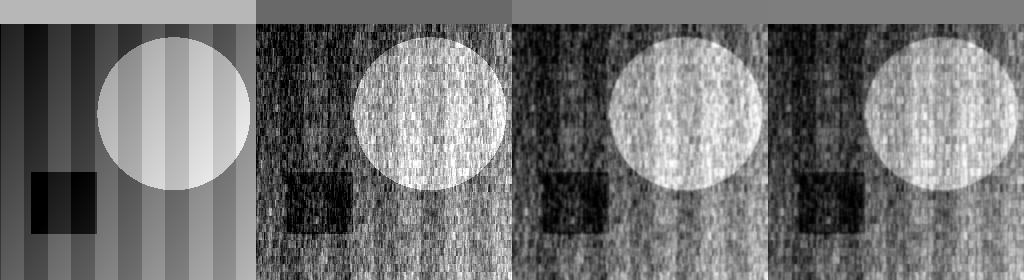
\includegraphics[width=\textwidth]{results/card_demo.png}
  \caption{CARD demonstration output. Left to right: clean image, correlated
  noisy image, Gaussian baseline, and CARD-style restoration.}
  \label{fig:card-result}
\end{figure}

\begin{table}[h]
  \centering
  \begin{tabular}{lcc}
    \toprule
    Image & PSNR & SSIM \\
    \midrule
    Correlated noisy & 18.62 & 0.889 \\
    Gaussian baseline & 22.07 & 0.946 \\
    CARD-style restore & 22.39 & 0.949 \\
    \bottomrule
  \end{tabular}
  \caption{Measured restoration quality in the deterministic demo.}
\end{table}

The CARD-style method improves over both the noisy image and the Gaussian
baseline in this experiment. The improvement is small but demonstrates the
benefit of using the covariance structure instead of ignoring correlation.

\section{Differences from the Original Paper}

\begin{table}[h]
  \centering
  \small
  \resizebox{\textwidth}{!}{%
  \begin{tabular}{lll}
    \toprule
    Component & Original CARD & This Project \\
    \midrule
    Restoration engine & DDRM diffusion sampler & Wiener-style denoising \\
    Learned prior & Pretrained diffusion model & Gaussian image prior \\
    Tasks & Denoising, deblurring, super-resolution & Denoising only \\
    Noise data & Synthetic and real CIN-D & Synthetic only \\
    Covariance & Dark frames or synthetic model & Hand-designed synthetic model \\
    Evaluation & ImageNet, LSUN, CIN-D & One deterministic demo \\
    \bottomrule
  \end{tabular}
  }
  \caption{Comparison between the original paper and this implementation.}
\end{table}

\section{Limitations}

This implementation is intentionally simplified. Its main limitations are:

\begin{itemize}
  \item it does not implement the full DDRM diffusion sampler;
  \item it does not use a pretrained diffusion model;
  \item it does not estimate covariance from real dark frames;
  \item it only demonstrates denoising;
  \item it evaluates on a synthetic image rather than real sensor data;
  \item its SSIM calculation is a simple global metric.
\end{itemize}

\section{Conclusion}

The CARD paper shows that explicitly modeling correlated noise can improve image
restoration. This project demonstrates the same principle in a compact and
reproducible form. By constructing a covariance matrix, generating correlated
noise, and restoring in a covariance-aware representation, the implementation
shows why the i.i.d. noise assumption can be limiting and how covariance-aware
processing can improve restoration quality.

\end{document}
